\documentclass[12pt]{article}
%-------------------------------------------------------------------------------
\usepackage[paperwidth=50cm,voffset=-11pt,paperheight=35cm,margin=1cm]{geometry}
\usepackage{amsthm}
\usepackage{framed}
\usepackage{multicol}
\usepackage{lipsum,lineno}
\usepackage[backend=biber,sorting=none]{biblatex}
\addbibresource{referencias/Textos.bib}
\addbibresource{referencias/Articulos.bib}
\addbibresource{referencias/Libros.bib}
\usepackage[]{textpos}
\usepackage{multido}
\usepackage{ifthen}
\usepackage{xargs}
\usepackage{xparse}
\usepackage{color}
\usepackage{lipsum}  
\usepackage{caption}
\usepackage{lmodern}
\usepackage{mathtools,amsfonts}
\usepackage{enumitem}

\usepackage{xcolor}
\usepackage[spanish]{babel}
\usepackage{lipsum}
\usepackage{pgffor}

\usepackage[tikz]{bclogo}
\usepackage[most]{tcolorbox}
\usepackage{varwidth}
\usepackage{ifthen}
\usepackage{xparse}
\usepackage{pgfkeys}
\usetikzlibrary{calc}
\usepackage[explicit]{titlesec}
\usepackage{titletoc}
\usepackage{anyfontsize}
\usepackage{wrapfig}
\usepackage{minted}
\usepackage[inkscapearea=page]{svg}
\setsvg{inkscapeexe={"D:/software/programas/inkscape/bin/inkscape.exe"}}
\usepackage{xfakebold}

\RequirePackage{tcolorbox}
\usetikzlibrary{patterns}

\colorlet{CLinea}{gray!70!white}
\colorlet{CFondo}{gray!5!white}
\colorlet{CBlanco}{white}
\colorlet{CNegro}{black}

\colorlet{CFNombre}{red!80!white}
\colorlet{CBNombre}{red!10!white}

\colorlet{CTituloDeParrafo}{blue!40}
\colorlet{CSubrayadoDeTitulo}{blue!40}

\newcommand{\ConfigurarPaleta}{
%------------COMUNIDAD-----------------
\ifthenelse{\equal{\MODO}{ModoC}}
    {
    \colorlet{CFNombre}{green!80!white}
    \colorlet{CBNombre}{green!10!white}
    \colorlet{CTSeccion}{blue!40}
    \colorlet{CCSeccion}{gray!20}
    \definecolor{CTDiario}{RGB}{133, 146, 158}
    \definecolor{CCDiario}{RGB}{253, 254, 254}
    }{}
%-------------ESTUDIANTES-------------
\ifthenelse{\equal{\MODO}{ModoE}}
    {
    \colorlet{CFNombre}{yellow!80!white}
    \colorlet{CBNombre}{yellow!10!white}    
    \colorlet{CTSeccion}{blue!30}
    \definecolor{CCSeccion}{RGB}{255, 220, 110}   
    \definecolor{CTDiario}{RGB}{133, 193, 233}
    \definecolor{CCDiario}{RGB}{253, 242, 233}
    }{}
}

\usepackage{fontspec}
\usepackage[outline]{contour}
%------------------------CONFIGURARA FUENTES---------------------------
\newcommand{\FuenteTSG}{\fontsize{50}{50}}
\newcommand{\FuenteTG}{\fontsize{40}{40}}  
\newcommand{\FuenteTM}{\large}
\newcommand{\FuenteTP}{\normalsize} 

\newcommand{\FuenteComic}{ka Blam}
\newcommand{\FuenteEstudiante}{Just a Moment}
\newcommand{\FuenteDocente}{calibri}

\newcommand{\FUENTE}{\setmainfont{\FuenteEstudiante}}

\newcommand{\ConfigurarFuentes}{
  \ifthenelse{\equal{\MODO}{ModoE}}
             {%              
              \renewcommand{\FUENTE}{\setmainfont{\FuenteEstudiante}}           
             }{}
    \ifthenelse{\equal{\MODO}{ModoC}}
             {%            
              \renewcommand{\FUENTE}{\sffamily}            
             }{}    
}


\newcommand{\Escudo}{Escudo_UD}

\newcommand{\ConfigurarImagenes}{	
	%-------------ESTUDIANTES-------------
	\ifthenelse{\equal{\MODO}{ModoE}}
	{
	}{}
}


%%%%%%%%%%%%%%%%%%%%%%%%%%%%%%%%%%%%%%%%%%%%%%%%%%%%%%%%%%%%%%%%%%%%
%%%%%%%%%%%%%%%%%%%%%%%%%%%%% DISENO %%%%%%%%%%%%%%%%%%%%%%%%%%%%%%%
%%%%%%%%%%%%%%%%%%%%%%%%%%%%%%%%%%%%%%%%%%%%%%%%%%%%%%%%%%%%%%%%%%%%
\newcommand{\Comillas}[1]{``#1''}

\newcommand{\Negrita}[1]{
	 \ifthenelse{\equal{\MODO}{ModoE}}
	{% 
	\unskip\setBold[0.2]\aftergroup\unsetBold\aftergroup\ignorespaces  #1       
	}{}
	\ifthenelse{\equal{\MODO}{ModoC}}
	{%            
	 \textbf{#1}         
	}{}	
}

\newcommand{\COLOR}{\color{white}}
\newcommand{\MODO}{ModoD}
\newcommand{\MATERIA}{ARQUITECTURA EMPRESARIAL}
\newcommand{\Ciudad}{Bogotá}
\newcommand{\Volumen}{\date}

\newcommand{\Diario}[1]{	
	\FuenteTSG\color{CTDiario}\textbf{#1}	 
}

\titlecontents{section}[2.4pc]
{\addvspace{1pt}}
{\contentslabel[\thecontentslabel]{2.4pc}}
{}
{\dotfill\small \thecontentspage}
[]

\titleformat{\section}{\centering\bf\FuenteTG\COLOR}{\FuenteTG\bf\FUENTE\Alph{section}.#1}{0.5em}{}
%\newcommand{\titleformat{\subsection}{\centering\Large\selectfont\color{CTSeccion}}{\thesection}{0.5em}{}}
\newcommand{\subseccionC}[1]{
{\centering\FUENTE\Large\color{CTSeccion} \textbf{#1} \\ \vspace*{10pt} }
}
\newcommand{\subseccionI}[1]{
{\LARGE\selectfont\color{CTSeccion} #1 \\ \vspace*{10pt} }
}
%-----------------------DIBUJAR LINEA-------------------------------

\NewDocumentCommand{\DibujarLinea}{m m m m m}{
  \setlength{\parindent}{0cm}
  \setlength{\parskip}{0cm}
  %\noindent
  \count3=#1%
  \advance\count3 by 1%
   \multido{\i=0+1}{\count3}{       
        \ifthenelse{\equal{#5}{horizontal}}{
            %------horizontal
		  \begin{textblock}{#2}(0,\i)
			   \rule[0pt]{#3}{#4}
		  \end{textblock}
         }{
            %------vertical
            \begin{textblock}{#2}(\i,0)
			   \rule[0pt]{#3}{#4}
		    \end{textblock}
         }
	}
}

%------------------VARAIBLES GLOBALES-------------------------------

\newdimen\CeldaW
\newdimen\CeldaH
\newcount\nFilas
\newcount\nColus

%-----------------------CALCULAR GRILLA-----------------------------

\NewDocumentCommand{\CalcularGrilla}{m m O{\textwidth} O{\textheight} O{show}}
{
    %------variables------    
	\nFilas=#1 %filas
	\nColus=#2 %columnas	
    
    \CeldaW=#3 %ancho
    \CeldaH=#4 %alto
   %----------------------
	%calculoar celda
    \divide\CeldaH by \nFilas
	\divide\CeldaW by \nColus
	
	\setlength{\TPHorizModule}{\CeldaW}
	\setlength{\TPVertModule}{\CeldaH}
	
	\ifthenelse{\equal{#5}{show}}{
        %dibujar filas
		\DibujarLinea{\nFilas}{\nColus}{\textwidth}{.1pt}{horizontal}
        %dibujar columnas
        \DibujarLinea{\nColus}{\nFilas}{.1pt}{\textheight}{vertical}
	}{}	
}

%-----------------------NUEVA PAGINA-------------------------------

\NewDocumentEnvironment{NuevaPagina}{m m m}
{
 \thispagestyle{empty}
 \clearpage
 \CalcularGrilla{#1}{#2}[\textwidth][\textheight][#3]
}
%contenido
{
 \newpage
 }

 %-----------------------NUEVA PARRAFO-------------------------------
 %-----vvariables--------
 \newdimen\Margen
 \setlength{\Margen}{2pt}
 \newdimen\AltoP
 %------------------------
 \NewDocumentEnvironment{NuevoParrafo}{m m O{1} O{1}}%
 {%
 \setlength{\AltoP}{\dimexpr#4\TPVertModule-2\Margen\relax}%
 \TPMargin{\Margen}%
 \begin{textblock}{#3}(#2,#1)%
 }%
 {%  
 \end{textblock}%
 }%
%-------------------------------------------------------------------------------------------------------------%
%----------------------------------------CAJAS----------------------------------------------------------------%
%-------------------------------------------------------------------------------------------------------------%

\newcommand{\Imagen}[2]{   
    \ifthenelse{\equal{\MODO}{ModoE}}
    {%           
      \includesvg[#1]{formato/apariencia/imagenes/#2Cartoon}
    }{}
    \ifthenelse{\equal{\MODO}{ModoC}}
    {%            
      \includesvg[#1]{formato/apariencia/imagenes/#2}
    }{}   
}

\newcommand{\LineaIzqC}{0}
\newcommand{\LineaIzqU}{1}

\newcommand{\LineaDerC}{0}
\newcommand{\LineaDerU}{1}
\newcommand{\LineaDerD}{2}

\newcommand{\LineaSupC}{0}
\newcommand{\LineaSupU}{1}

\newcommand{\LineaInfC}{0}
\newcommand{\LineaInfU}{1}
\newcommand{\LineaInfD}{2}

\newcommand{\Vacio}{vacio}
\newcommand{\ADer}{right}
\newcommand{\AIzq}{left}
\newcommand{\Trazo}{0.3pt}
\newcommand{\Recta}{0.0pt}
\newcommand{\EspacioADer}{35pt}

\newcommand{\ConfigurarLineas}{
\ifthenelse{\equal{\MODO}{ModoE}}
           {\tikzset{decoration={random steps,segment length=5mm,amplitude=\Trazo}}}
           {\tikzset{decoration={random steps,segment length=5mm,amplitude=\Recta}}}
}
\tcbset{
	codigoMarco/.style n args={5}{
        empty,   
        height=\AltoP,        
        frame code={\path[fill=#5](frame.south west) rectangle (frame.north east);};
    	\ifthenelse{\equal{#1}{0}}{}{\draw[decorate,color=CLinea,line width =#1 pt](frame.north east) -- (frame.north west);};
    	\ifthenelse{\equal{#2}{0}}{}{\draw[decorate,color=CLinea,line width =#2 pt](frame.south east) -- (frame.south west);};
    	\ifthenelse{\equal{#3}{0}}{}{\draw[decorate,color=CLinea,line width =#3 pt](frame.north west) -- (frame.south west);};
        \ifthenelse{\equal{#4}{0}}{}{\draw[decorate,color=CLinea,line width =#4 pt](frame.north east) -- (frame.south east);};       
	}
}
\tcbset{
	codigoLinea/.style n args={1}{
		empty,   
		height=\AltoP,        
		frame code={\path[fill=white](frame.south west) rectangle (frame.north east);}; 
		{\draw[decorate,color=#1,line width =10pt]([yshift=-12pt]frame.north east) -- ([yshift=-12pt]frame.north west);};
	}   
 }
\newtcolorbox{Linea}[1]{%	
	codigoLinea={#1}
}

\newtcolorbox{MarcoSinTitulo}[5]{%	
    codigoMarco={#1}{#2}{#3}{#4}{#5}
}

\newtcolorbox{MarcoConTitulo}[8]{	
    title=#6,
    coltitle=CTituloDeParrafo,fonttitle=\normalsize,
    attach boxed title to top #7={yshift=-\tcboxedtitleheight,},    
    boxed title style={
    size=minimal, top=5pt,left=2pt,right=\EspacioADer,
    underlay={
              \draw[decorate,CSubrayadoDeTitulo,line width=3pt,] ([xshift=3pt,yshift=-5pt]frame.south west)--([xshift=-\EspacioADer,yshift=-5pt]frame.south east);
              \ifthenelse{\equal{#8}{\Vacio}}{}{\node[anchor=north east,outer sep=2pt] at ([yshift=2pt]frame.north east) {\includesvg[width=24pt]{#8}}};
             };
    },    
    %-------------------------------
    codigoMarco={#1}{#2}{#3}{#4}{#5}
}

\NewDocumentEnvironment{Marco}{O{1} O{1} O{1} O{1} O{CFondo} O{\Vacio} O{\Vacio} O{\Vacio}}%
{%
\ifthenelse{\equal{#8}{\Vacio}}
    {\renewcommand{\EspacioADer}{3pt}}
    {\renewcommand{\EspacioADer}{35pt}}%    
\ifthenelse{\equal{#6}{\Vacio}}
    {\begin{MarcoSinTitulo}{#1}{#2}{#3}{#4}{#5}}
    {\begin{MarcoConTitulo}{#1}{#2}{#3}{#4}{#5}{#6}{#7}{#8}\vspace*{20pt}}
}%
{
\ifthenelse{\equal{#6}{\Vacio}}
    {\end{MarcoSinTitulo}}
    {\end{MarcoConTitulo}}%
}%


%---------TITULO
\newcommand{\CabeceraDeSeccion}[4][30]{
\begin{NuevoParrafo}{0}{0}[#1][2]
	\begin{Marco}[\LineaSupU][\LineaInfD][\LineaIzqU][\LineaDerD][#4]
		\renewcommand{\COLOR}{\color{#3}}	
		\section{#2}  
	\end{Marco}
\end{NuevoParrafo}
}

\newcommand{\COLORSS}{\color{white}}
\titleformat{\subsection}{\centering\bf\LARGE\COLORSS}{\filcenter\LARGE\bf\FUENTE\Alph{subsection}.#1}{0.0em}{}
\titlecontents{subsection}[2.4pc]
{\addvspace{1pt}}
{---}
{}
{\dotfill\small \thecontentspage}
[]

\newcommand{\CabeceraDeSubSeccion}[4]{
	\begin{NuevoParrafo}{#1}{0}[8][1]
		\begin{Marco}[\LineaSupC][\LineaInfC][\LineaIzqC][\LineaDerC][CBlanco]
		    \begin{center}
		    	\vspace{-5pt}
		    	\renewcommand{\COLORSS}{\color{#3}}
		    	\subsection{#2}		    	
		    	%\color{#3}\LARGE#2
		    \end{center}		
		\end{Marco}
	\end{NuevoParrafo}
	\begin{NuevoParrafo}{#1}{7}[23][1]	
		\begin{Linea}{#4}
		\end{Linea}
	\end{NuevoParrafo}
}

\newcommand{\CabeceraDeSubSeccionConAncho}[5]{
	\begin{NuevoParrafo}{#1}{0}[8][1]
		\begin{Marco}[\LineaSupC][\LineaInfC][\LineaIzqC][\LineaDerC][CBlanco]
			\begin{center}
				\vspace{-5pt}
				\renewcommand{\COLORSS}{\color{#3}}
				\subsection{#2}		    	
				%\color{#3}\LARGE#2
			\end{center}		
		\end{Marco}
	\end{NuevoParrafo}
	\begin{NuevoParrafo}{#1}{7}[#5][1]	
		\begin{Linea}{#4}
		\end{Linea}
	\end{NuevoParrafo}
}

\newcommand{\CabeceraDeSubSeccionConAnchoN}[7]{
	\begin{NuevoParrafo}{#1}{#2}[16][2]
		\begin{Marco}[\LineaSupC][\LineaInfC][\LineaIzqC][\LineaDerC][CBlanco]
			\begin{center}
				\vspace{-5pt}
				\renewcommand{\COLORSS}{\color{#6}}
				\subsection{\textbf{#5}}		    	
				%\color{#3}\LARGE#2
			\end{center}		
		\end{Marco}
	\end{NuevoParrafo}
	\begin{NuevoParrafo}{#1}{\the\numexpr #2 + #3 \relax}[#4][1]	
		\begin{Linea}{#7}
		\end{Linea}
	\end{NuevoParrafo}
}

\newcommand{\SeparadorDeSubSeccion}[2]{	
	\begin{NuevoParrafo}{#1}{0}[30][1]	
		\begin{Linea}{#2}
		\end{Linea}
	\end{NuevoParrafo}
}

\newcommand{\CabeceraDePoster}[1]{
	\begin{NuevoParrafo}{0}{0}[8][6]
		\begin{Marco}[\LineaSupC][\LineaInfC][\LineaIzqC][\LineaDerC][CCDiario]
		\Imagen{width=65pt}{\Escudo}
		\end{Marco}
	\end{NuevoParrafo}	
	\begin{NuevoParrafo}{0}{8}[68][6]
		\begin{Marco}[\LineaSupC][\LineaInfC][\LineaIzqC][\LineaDerC][CCDiario]		  
		    \vspace{15pt}
		    \centering\FuenteTSG\color{CTDiario}\textbf{#1}							  
		\end{Marco}
	\end{NuevoParrafo}
}
\newcommand{\CiudadFechaVolumen}{
	\begin{NuevoParrafo}{6}{0}[94][2]
		\begin{Marco}[\LineaSupU][\LineaInfU][\LineaIzqC][\LineaDerC][CBlanco]
		\centering\Negrita{ --- \Ciudad\ \today\ \Volumen \ ---}
		\end{Marco}
	\end{NuevoParrafo}
}

\newcommand{\Pelicula}[3]{	
	\begin{minipage}[t]{9.2cm}
		\color{CTCine}{\Negrita{\large#1}}\begin{center}\includegraphics[width=5cm,height=6cm]{#2}\end{center}#3
	\end{minipage}
}

\newcommand{\Escritor}[3]{	
	\begin{minipage}[t]{18cm}
		\color{CTCine}{\Negrita{\large#1}}\\
		\begin{wrapfigure}{l}{0.3\textwidth}			
			\centering\includegraphics[width=4cm]{#2}			
		\end{wrapfigure}#3		
	\end{minipage}
}

\newcommand{\Personaje}[5]{	
	\begin{minipage}[t]{#1}
		\color{#2}{\Negrita{\large#3}}\\
		\begin{wrapfigure}{l}{4.5cm}			
			\centering\includegraphics[width=4cm]{#4}			
		\end{wrapfigure}#5		
	\end{minipage}
}

\newcommand{\SuperX}[3]{	
	\begin{minipage}[t]{29cm}
		\color{CTCine}{\Negrita{\large#1}}\\
		\begin{wrapfigure}{l}{0.2\textwidth}
			\vspace*{-20pt}			
			\centering\includegraphics[width=4cm]{#2}			
		\end{wrapfigure}#3		
	\end{minipage}
}

\newcommand*{\Obra}[1]{%
	\raisebox{-.3\baselineskip}{%
		\includegraphics[
		height=\baselineskip,
		width=\baselineskip,
		keepaspectratio,
		]{#1}%
	}%
}

\newcommand{\Libro}[2]{
		\begin{minipage}[t]{4.5cm}			
			\centering
			\includegraphics[width=3cm,height=4cm]{#1}\\{\small#2}
		\end{minipage}
	    \vspace{+\parskip}	
}%
\NewDocumentEnvironment{Libros}{m}%
{
\begin{minipage}[t]{11cm}
	\color{CTCine}{\Negrita{\large#1}}\newline\newline	
	\centering\hfill
}%
{
\end{minipage}
}%

%------------------------CONFIURACION DEL MODO-----------------------------------
%\input{formato/progsPython}
\newcommand{\Configuracion}[1]{
    \renewcommand{\MODO}{#1}%para elgir galeria
    \ConfigurarFuentes
    \FUENTE
    \ConfigurarLineas
    \ConfigurarPaleta    
    \ConfigurarImagenes    
}

\newcommand{\ciclolipsum}[1]{
\foreach \x in {1,...,#1}
{
	\lipsum[1][5]
}
\par
}
\newcommand{\cortelipsum}{
\vfill\null	
\columnbreak 
}
\newcommand{\nuevalinea}{\leavevmode\\}

\def\ImagenCircular[#1]#2#3{
	\begin{tikzpicture}
		\clip (0,0) circle (#1);
		\node (0,0) {\includegraphics[width=#2]{#3}};
	\end{tikzpicture}%
}

\newcommand{\autores}[3]{ 
\vspace{-5pt}
\large \centering{UNIVERSIDAD DISTRITAL FJC}
\vspace{5pt}
\hrule
\vspace{5pt}
 #1\\#2 \\#3
}

\newenvironment{MisionVision}[1][Mision]{ 
	\begin{minipage}[t][.20\textheight]{\textwidth}
		\begin{center}
			\color{gray}\bfseries{\fontsize{20}{10}\selectfont #1}
			\vspace{-10pt}
			%\subsubsection{#1}
		\end{center}	
	}
{
	\end{minipage}\\[1cm]
}
\newenvironment{Vision}[1][Vision]{ 
	\begin{minipage}[t][.20\textheight]{\textwidth}
		\begin{center}
			%\color{gray}\bfseries{\fontsize{25}{10}\selectfont #1}
			\section{#1}
		\end{center}	
	}
	{
	\end{minipage}\\[2cm]
}
\newenvironment{Objetivos}[1][Objetivos]{ 
	\begin{minipage}[t][.20\textheight]{\textwidth}
		\begin{center}
			\color{gray}\bfseries{\fontsize{20}{10}\selectfont #1}
			\vspace{-18pt}
			%\color{gray}\bfseries{\fontsize{25}{10}\selectfont #1}
			%\section{#1}
		\end{center}	
	}
	{
	\end{minipage}\\[1cm]
}
%-----------------CONSTANTES--------------------
\newcommand{\PVD}{Punto de Vista de\ }
\newcommand{\PV}{Punto de Vista \ }
%-------------------------------------------------------------------
\newcommand{\PVSta}{Stakeholder}
\newcommand{\PVROb}{Realización de Objetivos}
\newcommand{\PVCOb}{Contribución de Objetivos}
\newcommand{\PVPri}{Principios}
\newcommand{\PVReR}{Realización de Requerimientos}
\newcommand{\PVMot}{Motivación}

\newcommand{\PVOrg}{Organizacion}
\newcommand{\PVCAc}{Cooperacion de Actor}
\newcommand{\PVFNe}{Función de Negocio}
\newcommand{\PVPNe}{Proceso de Negocio}
\newcommand{\PVCPN}{Cooperacion de Proceso de Negocio }
\newcommand{\PVPro}{Producto}

\newcommand{\Org}{Organizacion}
\newcommand{\CoA}{CoopActor}
\newcommand{\FNe}{FuncionNegocio}
\newcommand{\PNe}{ProcesoNegocio}
\newcommand{\CPN}{CoopProcesoNegocio}
\newcommand{\Pro}{Producto}

\newcommand{\PVCMA}{Comportamiento de Aplicación}
\newcommand{\PVCOA}{Cooperación de Aplicación}
\newcommand{\PVEAp}{Estructura de Aplicación}
\newcommand{\PVUAp}{Uso de Aplicación}

\newcommand{\CAp}{CmtoAplicacion}
\newcommand{\CpA}{CoopAplicacion}
\newcommand{\EsA}{EstrAplicacion}
\newcommand{\UsA}{UsoAplicacion}

\newcommand{\PVTec}{Tecnología}
\newcommand{\PVUTe}{Uso de Tecnología}
\newcommand{\PVDIm}{Despliegue e Implementación}
\newcommand{\PVEIn}{Estructura de Información}
\newcommand{\PVRSe}{Realización del Servicio}
\newcommand{\PVFis}{Fisico}
\newcommand{\PVCap}{Capas}

\newcommand{\Tec}{Tecnologia}
\newcommand{\UsT}{UsoTecnologia}
\newcommand{\Imp}{Implementacion}
\newcommand{\EsI}{EstrInformacion}
\newcommand{\ReS}{RealServicio}
\newcommand{\Fis}{Fisico}
\newcommand{\Cap}{Capas}



\newcommand{\Int}{Interesado}
\newcommand{\ReO}{RealObjetivos}
\newcommand{\CoO}{ContObjetivos}
\newcommand{\Pri}{Principios}
\newcommand{\ReR}{RealRequerimientos}
\newcommand{\Mot}{Motivacion}

\newcommand{\PVPry}{Proyecto}
\newcommand{\PVMig}{Migraión}
\newcommand{\PVImM}{Imp/Migración}

\newcommand{\Pry}{Proyecto}
\newcommand{\Mig}{Migracion}
\newcommand{\ImM}{ImplementacionMigracion}

\newcommand{\PVEtg}{Estrategia}
\newcommand{\PVMaC}{Mapa de Capacidad}
\newcommand{\PVRes}{Realización de Resultado}
\newcommand{\PVMaR}{Mapa de Recurso}
\newcommand{\PVFdV}{Flujo de Valor}

\newcommand{\Etg}{Estrategia}
\newcommand{\MaC}{MapaCapacidad}
\newcommand{\Res}{RealResultado}
\newcommand{\MaR}{MapaRecurso}
\newcommand{\FdV}{FlujoDeValor}


\newcommand{\RMe}{imgs/meta/}
\newcommand{\RM}{imgs/modelo/}
\newcommand{\RC}{imgs/caso/}
\renewcommand*\familydefault{\sfdefault}
%--------------------------------------------------------------------------------
\begin{document}
\Configuracion{ModoE}
\begin{NuevaPagina}{64}{94}{show1}
	%------------------------------CABECERA----------------------------
	\CabeceraDePoster{\MATERIA} 
	\begin{NuevoParrafo}{0}{76}[18][6]
		\begin{Marco}[\LineaSupC][\LineaInfC][\LineaIzqC][\LineaDerC][CBlanco]
			\autores{Sergio Cardenas - Cod:20192020126}{Stivel Pinilla - Cod:20191020024}{Juan Mancera - Cod:20171020047}
		\end{Marco}
	\end{NuevoParrafo} 
	%-------------------------------DIVISION--------------------------
	\CiudadFechaVolumen
	%----------------------------MISION/VISION------------------------
	\CabeceraDeSubSeccionConAnchoN{9}{0}{14}{80}{FARMA-WEB}{CTDiario}{CCDiario}
	\begin{NuevoParrafo}{11}{0}[46][6]
		\begin{Marco}[\LineaSupC][\LineaInfC][\LineaIzqC][\LineaDerC][CBlanco]
			\begin{MisionVision}[Misión]
				{Desarrollar soluciones tecnológicas innovadoras de monitoreo y análisis de la calidad del aire que integren ciencia de datos y usabilidad, con el fin de proporcionar información clara, confiable y accesible a la ciudadanía de Bogotá, a las entidades ambientales y a la comunidad científica. Nuestro compromiso es impulsar decisiones más conscientes y políticas públicas efectivas que promuevan un ambiente más saludable y sostenible.}
			\end{MisionVision}			
		\end{Marco}
	\end{NuevoParrafo}
	%\CabeceraDeSubSeccionConAnchoN{4}{0}{7}{39}{FARMA-WEB}{CTDiario}{CCDiario}
	\begin{NuevoParrafo}{17}{0}[46][6]
		\begin{Marco}[\LineaSupC][\LineaInfC][\LineaIzqC][\LineaDerC][CBlanco]
			\begin{MisionVision}[Visión]
				{Ser en el año 2030 la empresa líder en Colombia en el desarrollo de software de calidad del aire, reconocida por su impacto en la toma de decisiones ambientales, su aporte a la investigación científica y su capacidad de empoderar a la ciudadanía con herramientas digitales que contribuyan a mejorar la salud pública y la sostenibilidad urbana.}
			\end{MisionVision}
		\end{Marco}
	\end{NuevoParrafo}
		\begin{NuevoParrafo}{11}{48}[46][12]
		\begin{Marco}[\LineaSupC][\LineaInfC][\LineaIzqC][\LineaDerC][CBlanco]
			\begin{Objetivos}[Objetivos]
				{	{\large General:}\vspace{5pt}\\
					{\linespread{.8}\selectfont Desarrollar un software de monitoreo y análisis de la calidad del aire en Bogotá que integre datos ambientales de distintas fuentes oficiales, brinde visualizaciones intuitivas y facilite la toma de decisiones informadas por parte de la ciudadanía, las entidades gubernamentales y la comunidad científica.}\\[0.3cm]
					{\large Específicos:}
					{\begin{itemize}
							\setlength{\itemsep}{-0.5pt}
							\setlength{\parskip}{0pt}
							\setlength{\parsep}{0pt}
							\item Diseñar una plataforma digital con interfaces accesibles y usables que permitan a los usuarios finales consultar información clara y confiable sobre la calidad del aire en tiempo real.
							\item Implementar modelos de análisis de datos e indicadores ambientales que apoyen la formulación de políticas públicas, investigaciones científicas y programas de educación ambiental en Bogotá.
					\end{itemize}}
				}
			\end{Objetivos}
		\end{Marco}
	\end{NuevoParrafo}
	
	%----------------CAPA DE MOTIVACION------------------------------------------	
	
	\CabeceraDeSubSeccionConAnchoN{23}{0}{14}{80}{MOTIVACION}{CTDiario}{CCDiario}
	\begin{NuevoParrafo}{26}{41}[26][15]
		\begin{Marco}[\LineaSupC][\LineaInfC][\LineaIzqC][\LineaDerC][CBlanco]
		\subseccionC{\PVSta}%{CTSeccionPrimeraPlana}{CCSeccionPrimeraPlana} 
		\centering\includegraphics[scale=0.68]{\RC/motivacion/Interesado.pdf}
		\end{Marco}
	\end{NuevoParrafo}

	%-----------------------------ORIGINAL---------------------------------------------
	% \begin{NuevoParrafo}{26}{0}[40][20]
	% 	\begin{Marco}[\LineaSupC][\LineaInfC][\LineaIzqC][\LineaDerC][CBlanco]
	% 		\subseccionC{MetaModelo}%{CTSeccionPrimeraPlana}{CCSeccionPrimeraPlana} 
	% 		\centering\includegraphics[scale=0.68]{\RMe MetaMotivacion.pdf}
	% 	\end{Marco}
	% \end{NuevoParrafo}
	
	% \begin{NuevoParrafo}{26}{41}[26][15]
	% 	\begin{Marco}[\LineaSupC][\LineaInfC][\LineaIzqC][\LineaDerC][CBlanco]
	% 	\subseccionC{\PVSta}%{CTSeccionPrimeraPlana}{CCSeccionPrimeraPlana} 
	% 	\centering\includegraphics[scale=0.68]{\RC/motivacion/Interesado.pdf}
	% 	\end{Marco}
	% \end{NuevoParrafo}
	
	% \begin{NuevoParrafo}{26}{68}[26][15]
	% 	\begin{Marco}[\LineaSupC][\LineaInfC][\LineaIzqC][\LineaDerC][CBlanco]
	% 		\subseccionC{\PVPri}%{CTSeccionPrimeraPlana}{CCSeccionPrimeraPlana} 
	% 		\centering\includegraphics[scale=0.68]{\RC/motivacion/Principios.pdf}
	% 	\end{Marco}
	% \end{NuevoParrafo}
	
	% \begin{NuevoParrafo}{47}{0}[20][15]
	% 	\begin{Marco}[\LineaSupC][\LineaInfC][\LineaIzqC][\LineaDerC][CBlanco]
	% 		\subseccionC{\PVROb}%{CTSeccionPrimeraPlana}{CCSeccionPrimeraPlana} 
	% 		\centering\includegraphics[scale=0.64]{\RC/motivacion/RealObjetivos.pdf}
	% 	\end{Marco}
	% \end{NuevoParrafo}
	
	
	% \begin{NuevoParrafo}{47}{20}[20][15]
	% 	\begin{Marco}[\LineaSupC][\LineaInfC][\LineaIzqC][\LineaDerC][CBlanco]
	% 		\subseccionC{\PVCOb}%{CTSeccionPrimeraPlana}{CCSeccionPrimeraPlana} 
	% 		\centering\includegraphics[scale=0.68]{\RC/motivacion/ContObjetivos.pdf}
	% 	\end{Marco}
	% \end{NuevoParrafo}
	
	
	% \begin{NuevoParrafo}{45}{41}[26][17]
	% 	\begin{Marco}[\LineaSupC][\LineaInfC][\LineaIzqC][\LineaDerC][CBlanco]
	% 		\subseccionC{\PVReR}%{CTSeccionPrimeraPlana}{CCSeccionPrimeraPlana} 
	% 		\centering\includegraphics[scale=0.68]{\RC/motivacion/RealRequerimientos.pdf}
	% 	\end{Marco}
	% \end{NuevoParrafo}
	% \begin{NuevoParrafo}{45}{68}[26][17]
	% 	\begin{Marco}[\LineaSupC][\LineaInfC][\LineaIzqC][\LineaDerC][CBlanco]
	% 		\subseccionC{\PVMot}%{CTSeccionPrimeraPlana}{CCSeccionPrimeraPlana} 
	% 		\centering\includegraphics[scale=0.68]{\RC/motivacion/Motivacion.pdf}
	% 	\end{Marco}
	% \end{NuevoParrafo}

%%%%%%%%%%%%%%%%%%%%%%%%%%%%%%%%%%%%%%%%%%%%%%%%%%%%%%%%%%%%%%%%%%%%%%%%%%%%%%%%%%%%%%
\end{NuevaPagina}
\begin{NuevaPagina}{64}{94}{show1}
	%------------------------------CABECERA----------------------------
	\CabeceraDePoster{\MATERIA} 
	\begin{NuevoParrafo}{0}{76}[18][6]
		\begin{Marco}[\LineaSupC][\LineaInfC][\LineaIzqC][\LineaDerC][CBlanco]
			\autores{Sergio Cardenas - Cod:20192020126}{Stivel Pinilla - Cod:20191020024}{Juan Mancera - Cod:20171020047}
		\end{Marco}
	\end{NuevoParrafo} 
	%-------------------------------DIVISION--------------------------
	\CiudadFechaVolumen
	
	%----------------CAPA DE ESTRATEGIA------------------------------------------	
	\CabeceraDeSubSeccionConAnchoN{9}{0}{14}{80}{ESTRATEGIA}{CTDiario}{CCDiario}
	\begin{NuevoParrafo}{11}{0}[22][12]
		\begin{Marco}[\LineaSupC][\LineaInfC][\LineaIzqC][\LineaDerC][CBlanco]
			\subseccionC{MetaModelo}%{CTSeccionPrimeraPlana}{CCSeccionPrimeraPlana} 
			\centering\includegraphics[scale=0.68]{\RMe MetaEstrategia.pdf}		
		\end{Marco}
	\end{NuevoParrafo}	
	\begin{NuevoParrafo}{11}{23}[16][12]
		\begin{Marco}[\LineaSupC][\LineaInfC][\LineaIzqC][\LineaDerC][CBlanco]
			\subseccionC{\PVMaC}%{CTSeccionPrimeraPlana}{CCSeccionPrimeraPlana} 
			\centering\includegraphics[scale=0.6]{\RCR/estrategia/Capacidad.pdf}		
		\end{Marco}
	\end{NuevoParrafo}	
	\begin{NuevoParrafo}{23}{23}[16][11]
		\begin{Marco}[\LineaSupC][\LineaInfC][\LineaIzqC][\LineaDerC][CBlanco]
			\subseccionC{\PVMaR}%{CTSeccionPrimeraPlana}{CCSeccionPrimeraPlana} 
			\centering\includegraphics[scale=0.46]{\RCR/estrategia/Recursos.pdf}		
		\end{Marco}
	\end{NuevoParrafo}	
		\begin{NuevoParrafo}{23}{40}[22][11]
		\begin{Marco}[\LineaSupC][\LineaInfC][\LineaIzqC][\LineaDerC][CBlanco]
			\subseccionC{\PVFdV}%{CTSeccionPrimeraPlana}{CCSeccionPrimeraPlana} 
			\centering\includegraphics[scale=0.45]{\RCR/estrategia/Flujo_Valor.pdf}		
		\end{Marco}
	\end{NuevoParrafo}	
	\begin{NuevoParrafo}{11}{40}[22][12]
		\begin{Marco}[\LineaSupC][\LineaInfC][\LineaIzqC][\LineaDerC][CBlanco]
			\subseccionC{\PVRes}%{CTSeccionPrimeraPlana}{CCSeccionPrimeraPlana} 
			\centering\includegraphics[scale=0.35]{\RCR/estrategia/Realizacion_Resultados.pdf}		
		\end{Marco}
	\end{NuevoParrafo}	

	\begin{NuevoParrafo}{11}{63}[31][23]
		\begin{Marco}[\LineaSupC][\LineaInfC][\LineaIzqC][\LineaDerC][CBlanco]
			\subseccionC{\PVEtg}%{CTSeccionPrimeraPlana}{CCSeccionPrimeraPlana} 
			\centering\includegraphics[scale=0.65]{\RCR/estrategia/Estrategia.pdf}		
		\end{Marco}
	\end{NuevoParrafo}	
	% \begin{NuevoParrafo}{11}{23}[16][12]
	% 	\begin{Marco}[\LineaSupC][\LineaInfC][\LineaIzqC][\LineaDerC][CBlanco]
	% 		\subseccionC{\PVMaC}%{CTSeccionPrimeraPlana}{CCSeccionPrimeraPlana} 
	% 		\centering\includegraphics[scale=0.68]{\RC/estrategia/MapaCapacidad.pdf}		
	% 	\end{Marco}
	% \end{NuevoParrafo}	
	% \begin{NuevoParrafo}{23}{23}[16][11]
	% 	\begin{Marco}[\LineaSupC][\LineaInfC][\LineaIzqC][\LineaDerC][CBlanco]
	% 		\subseccionC{\PVMaR}%{CTSeccionPrimeraPlana}{CCSeccionPrimeraPlana} 
	% 		\centering\includegraphics[scale=0.68]{\RC/estrategia/MapaRecurso.pdf}		
	% 	\end{Marco}
	% \end{NuevoParrafo}	
	% 	\begin{NuevoParrafo}{23}{40}[22][11]
	% 	\begin{Marco}[\LineaSupC][\LineaInfC][\LineaIzqC][\LineaDerC][CBlanco]
	% 		\subseccionC{\PVFdV}%{CTSeccionPrimeraPlana}{CCSeccionPrimeraPlana} 
	% 		\centering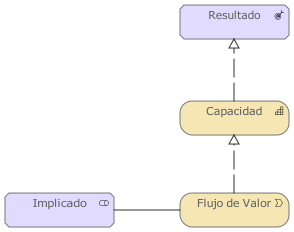
\includegraphics[scale=0.6]{\RC/estrategia/FlujoDeValor.pdf}		
	% 	\end{Marco}
	% \end{NuevoParrafo}	
	% \begin{NuevoParrafo}{11}{40}[22][12]
	% 	\begin{Marco}[\LineaSupC][\LineaInfC][\LineaIzqC][\LineaDerC][CBlanco]
	% 		\subseccionC{\PVRes}%{CTSeccionPrimeraPlana}{CCSeccionPrimeraPlana} 
	% 		\centering\includegraphics[scale=0.68]{\RC/estrategia/RealResultado.pdf}		
	% 	\end{Marco}
	% \end{NuevoParrafo}	

	% \begin{NuevoParrafo}{11}{63}[31][23]
	% 	\begin{Marco}[\LineaSupC][\LineaInfC][\LineaIzqC][\LineaDerC][CBlanco]
	% 		\subseccionC{\PVEtg}%{CTSeccionPrimeraPlana}{CCSeccionPrimeraPlana} 
	% 		\centering\includegraphics[scale=0.68]{\RC/estrategia/Estrategia.pdf}		
	% 	\end{Marco}
	% \end{NuevoParrafo}	
	%----------------CAPA DE NEGOCIO------------------------------------------	
	\CabeceraDeSubSeccionConAnchoN{34}{0}{14}{80}{NEGOCIO}{CTDiario}{CCDiario}
	\begin{NuevoParrafo}{36}{0}[40][16]
		\begin{Marco}[\LineaSupC][\LineaInfC][\LineaIzqC][\LineaDerC][CBlanco]
			\subseccionC{MetaModelo}%{CTSeccionPrimeraPlana}{CCSeccionPrimeraPlana} 
			\centering\includegraphics[scale=0.68]{\RMe MetaNegocio.pdf}
		\end{Marco}
	\end{NuevoParrafo}
	
	\begin{NuevoParrafo}{36}{41}[26][11]
		\begin{Marco}[\LineaSupC][\LineaInfC][\LineaIzqC][\LineaDerC][CBlanco]
			\subseccionC{\PVOrg}%{CTSeccionPrimeraPlana}{CCSeccionPrimeraPlana} 
			\centering\includegraphics[scale=0.55]{\RCR/negocio/Organizacion.pdf}
		\end{Marco}
	\end{NuevoParrafo}
	
	\begin{NuevoParrafo}{36}{68}[26][15]
		\begin{Marco}[\LineaSupC][\LineaInfC][\LineaIzqC][\LineaDerC][CBlanco]
			\subseccionC{\PVCAc}%{CTSeccionPrimeraPlana}{CCSeccionPrimeraPlana} 
			\centering\includegraphics[scale=0.65]{\RCR/negocio/Cooperacion_Actor.pdf}
		\end{Marco}
	\end{NuevoParrafo}
	
	\begin{NuevoParrafo}{52}{0}[20][12]
		\begin{Marco}[\LineaSupC][\LineaInfC][\LineaIzqC][\LineaDerC][CBlanco]
			\subseccionC{\PVPNe}%{CTSeccionPrimeraPlana}{CCSeccionPrimeraPlana}		
			\centering\includegraphics[scale=0.55]{\RCR/negocio/Proceso_Negocio.pdf}
		\end{Marco}
	\end{NuevoParrafo}
	
	\begin{NuevoParrafo}{52}{20}[20][12]
		\begin{Marco}[\LineaSupC][\LineaInfC][\LineaIzqC][\LineaDerC][CBlanco]
			\subseccionC{\PVCPN}%{CTSeccionPrimeraPlana}{CCSeccionPrimeraPlana}			
			\centering\includegraphics[scale=0.55]{\RCR/negocio/Cooperacion_Proceso.pdf}
		\end{Marco}
	\end{NuevoParrafo}
	
	
	\begin{NuevoParrafo}{48}{41}[26][16]
		\begin{Marco}[\LineaSupC][\LineaInfC][\LineaIzqC][\LineaDerC][CBlanco]
			\subseccionC{\PVFNe}%{CTSeccionPrimeraPlana}{CCSeccionPrimeraPlana} 
			\centering\includegraphics[scale=0.55]{\RCR/negocio/Funcion_Negocio.pdf}
		\end{Marco}
	\end{NuevoParrafo}
	\begin{NuevoParrafo}{52}{68}[26][12]
		\begin{Marco}[\LineaSupC][\LineaInfC][\LineaIzqC][\LineaDerC][CBlanco]
			\subseccionC{\Pro}%{CTSeccionPrimeraPlana}{CCSeccionPrimeraPlana} 
			\centering\includegraphics[scale=0.65]{\RCR/negocio/Producto.pdf}
		\end{Marco}
	\end{NuevoParrafo}

	% \begin{NuevoParrafo}{36}{41}[26][11]
	% 	\begin{Marco}[\LineaSupC][\LineaInfC][\LineaIzqC][\LineaDerC][CBlanco]
	% 		\subseccionC{\PVOrg}%{CTSeccionPrimeraPlana}{CCSeccionPrimeraPlana} 
	% 		\centering\includegraphics[scale=0.68]{\RC/negocio/Organizacion.pdf}
	% 	\end{Marco}
	% \end{NuevoParrafo}
	
	% \begin{NuevoParrafo}{36}{68}[26][15]
	% 	\begin{Marco}[\LineaSupC][\LineaInfC][\LineaIzqC][\LineaDerC][CBlanco]
	% 		\subseccionC{\PVCAc}%{CTSeccionPrimeraPlana}{CCSeccionPrimeraPlana} 
	% 		\centering\includegraphics[scale=0.68]{\RC/negocio/CoopActor.pdf}
	% 	\end{Marco}
	% \end{NuevoParrafo}
	
	% \begin{NuevoParrafo}{52}{0}[20][12]
	% 	\begin{Marco}[\LineaSupC][\LineaInfC][\LineaIzqC][\LineaDerC][CBlanco]
	% 		\subseccionC{\PVPNe}%{CTSeccionPrimeraPlana}{CCSeccionPrimeraPlana}		
	% 		\centering\includegraphics[scale=0.68]{\RC/negocio/ProcesoNegocio.pdf}
	% 	\end{Marco}
	% \end{NuevoParrafo}
	
	% \begin{NuevoParrafo}{52}{20}[20][12]
	% 	\begin{Marco}[\LineaSupC][\LineaInfC][\LineaIzqC][\LineaDerC][CBlanco]
	% 		\subseccionC{\PVCPN}%{CTSeccionPrimeraPlana}{CCSeccionPrimeraPlana}			
	% 		\centering\includegraphics[scale=0.68]{\RC/negocio/CoopProcesoNegocio.pdf}
	% 	\end{Marco}
	% \end{NuevoParrafo}
	
	
	% \begin{NuevoParrafo}{48}{41}[26][16]
	% 	\begin{Marco}[\LineaSupC][\LineaInfC][\LineaIzqC][\LineaDerC][CBlanco]
	% 		\subseccionC{\PVFNe}%{CTSeccionPrimeraPlana}{CCSeccionPrimeraPlana} 
	% 		\centering\includegraphics[scale=0.64]{\RC/negocio/FuncionNegocio.pdf}
	% 	\end{Marco}
	% \end{NuevoParrafo}
	% \begin{NuevoParrafo}{52}{68}[26][12]
	% 	\begin{Marco}[\LineaSupC][\LineaInfC][\LineaIzqC][\LineaDerC][CBlanco]
	% 		\subseccionC{\Pro}%{CTSeccionPrimeraPlana}{CCSeccionPrimeraPlana} 
	% 		\centering\includegraphics[scale=0.68]{\RC/negocio/Producto.pdf}
	% 	\end{Marco}
	% \end{NuevoParrafo}
	
	%%%%%%%%%%%%%%%%%%%%%%%%%%%%%%%%%%%%%%%%%%%%%%%%%%%%%%%%%%%%%%%%%%%%%%%%%%%%%%%%%%%%%%
\end{NuevaPagina}
\begin{NuevaPagina}{64}{94}{show1}
	%------------------------------CABECERA----------------------------
	\CabeceraDePoster{\MATERIA} 
	\begin{NuevoParrafo}{0}{76}[18][6]
		\begin{Marco}[\LineaSupC][\LineaInfC][\LineaIzqC][\LineaDerC][CBlanco]
			\autores{sandro Bolaños cod 202400000}{Javier Castro cod 202400000}
		\end{Marco}
	\end{NuevoParrafo} 
	%-------------------------------DIVISION--------------------------
	\CiudadFechaVolumen
	%----------------------------MISION/VISION------------------------
	\CabeceraDeSubSeccionConAnchoN{9}{0}{14}{80}{ESTRATEGIA}{CTDiario}{CCDiario}
	\begin{NuevoParrafo}{11}{0}[22][14]
		\begin{Marco}[\LineaSupC][\LineaInfC][\LineaIzqC][\LineaDerC][CBlanco]
			\subseccionC{MetaModelo}%{CTSeccionPrimeraPlana}{CCSeccionPrimeraPlana} 
			\centering\includegraphics[scale=0.60]{\RMe MetaAplicacion.pdf}		
		\end{Marco}
	\end{NuevoParrafo}	
	\begin{NuevoParrafo}{11}{22}[14][14]
		\begin{Marco}[\LineaSupC][\LineaInfC][\LineaIzqC][\LineaDerC][CBlanco]
			\subseccionC{\PVUAp}%{CTSeccionPrimeraPlana}{CCSeccionPrimeraPlana} 
			\centering\includegraphics[scale=0.60]{\RC/aplicacion/UsoAplicacion.pdf}		
		\end{Marco}
	\end{NuevoParrafo}	
	
	\begin{NuevoParrafo}{11}{57}[21][14]
		\begin{Marco}[\LineaSupC][\LineaInfC][\LineaIzqC][\LineaDerC][CBlanco]
			\subseccionC{\PVCMA}%{CTSeccionPrimeraPlana}{CCSeccionPrimeraPlana} 
			\centering\includegraphics[scale=0.60]{\RC/aplicacion/CmtoAplicacion.pdf}		
		\end{Marco}
	\end{NuevoParrafo}	
	\begin{NuevoParrafo}{11}{36}[21][14]
		\begin{Marco}[\LineaSupC][\LineaInfC][\LineaIzqC][\LineaDerC][CBlanco]			
		\subseccionC{\PVEAp}%{CTSeccionPrimeraPlana}{CCSeccionPrimeraPlana} 
		\centering\includegraphics[scale=0.60]{\RC/aplicacion/EstrAplicacion.pdf}		
		\end{Marco}
	\end{NuevoParrafo}	
	
	\begin{NuevoParrafo}{11}{78}[16][14]
		\begin{Marco}[\LineaSupC][\LineaInfC][\LineaIzqC][\LineaDerC][CBlanco]
			\subseccionC{\PVCOA}%{CTSeccionPrimeraPlana}{CCSeccionPrimeraPlana} 
			\centering\includegraphics[scale=0.6]{\RC/aplicacion/CoopAplicacion.pdf}		
		\end{Marco}
	\end{NuevoParrafo}	
	%----------------CAPA DE MOTIVACION------------------------------------------	
	\CabeceraDeSubSeccionConAnchoN{25}{0}{14}{80}{TECNOLOGIA}{CTDiario}{CCDiario}
	\begin{NuevoParrafo}{27}{0}[36][16]
		\begin{Marco}[\LineaSupC][\LineaInfC][\LineaIzqC][\LineaDerC][CBlanco]
			\subseccionC{MetaModelo}%{CTSeccionPrimeraPlana}{CCSeccionPrimeraPlana} 
			\centering\includegraphics[scale=0.6]{\RMe MetaTecnologia.pdf}
		\end{Marco}
	\end{NuevoParrafo}
	
	\begin{NuevoParrafo}{27}{36}[18][12]
		\begin{Marco}[\LineaSupC][\LineaInfC][\LineaIzqC][\LineaDerC][CBlanco]
			\subseccionC{\PVTec}%{CTSeccionPrimeraPlana}{CCSeccionPrimeraPlana} 
			\centering\includegraphics[scale=0.68]{\RC/tecnologia/Tecnologia.pdf}
		\end{Marco}
	\end{NuevoParrafo}
	
	\begin{NuevoParrafo}{27}{54}[21][12]
		\begin{Marco}[\LineaSupC][\LineaInfC][\LineaIzqC][\LineaDerC][CBlanco]
			\subseccionC{\PVUTe}%{CTSeccionPrimeraPlana}{CCSeccionPrimeraPlana} 
			\centering\includegraphics[scale=0.68]{\RC/tecnologia/UsoTecnologia.pdf}
		\end{Marco}
	\end{NuevoParrafo}
	
	\begin{NuevoParrafo}{43}{0}[18][9]
		\begin{Marco}[\LineaSupC][\LineaInfC][\LineaIzqC][\LineaDerC][CBlanco]
			\subseccionC{\PVRSe}%{CTSeccionPrimeraPlana}{CCSeccionPrimeraPlana} 
			\centering\includegraphics[scale=0.6]{\RC/tecnologia/RealServicio.pdf}
			
		\end{Marco}
	\end{NuevoParrafo}
	
	\begin{NuevoParrafo}{43}{18}[18][9]
		\begin{Marco}[\LineaSupC][\LineaInfC][\LineaIzqC][\LineaDerC][CBlanco]
			\subseccionC{\PVFis}%{CTSeccionPrimeraPlana}{CCSeccionPrimeraPlana} 
			\centering\includegraphics[scale=0.68]{\RC/tecnologia/Fisico.pdf}
		\end{Marco}
	\end{NuevoParrafo}
	
	
	\begin{NuevoParrafo}{39}{36}[18][13]
		\begin{Marco}[\LineaSupC][\LineaInfC][\LineaIzqC][\LineaDerC][CBlanco]
			\subseccionC{\PVDIm}%{CTSeccionPrimeraPlana}{CCSeccionPrimeraPlana}		
			\centering\includegraphics[scale=0.68]{\RC/tecnologia/Implementacion.pdf}
		\end{Marco}
	\end{NuevoParrafo}
	\begin{NuevoParrafo}{39}{54}[21][13]
		\begin{Marco}[\LineaSupC][\LineaInfC][\LineaIzqC][\LineaDerC][CBlanco]			
			\subseccionC{\PVEIn}%{CTSeccionPrimeraPlana}{CCSeccionPrimeraPlana}			
			\centering\includegraphics[scale=0.68]{\RC/tecnologia/EstrInformacion.pdf}
		\end{Marco}
	\end{NuevoParrafo}
	
	\begin{NuevoParrafo}{27}{75}[19][25]
		\begin{Marco}[\LineaSupC][\LineaInfC][\LineaIzqC][\LineaDerC][CBlanco]			
			\subseccionC{\PVCap}%{CTSeccionPrimeraPlana}{CCSeccionPrimeraPlana}			
			\centering\includegraphics[scale=0.68]{\RC/tecnologia/Capas.pdf}
		\end{Marco}
	\end{NuevoParrafo}
	
	%%%%%%%%%%%%%%%%%%%%%%%%%%%%%%%%%%%%%%%%%%%%%%%%%%%%%%%%%%%%%%%%%%%%%%%%%%%%%%%%%%%%%%
	\CabeceraDeSubSeccionConAnchoN{52}{0}{14}{53}{PROYECTO}{CTDiario}{CCDiario}
	\begin{NuevoParrafo}{54}{0}[22][9]
		\begin{Marco}[\LineaSupC][\LineaInfC][\LineaIzqC][\LineaDerC][CBlanco]
			\subseccionC{MetaModelo}%{CTSeccionPrimeraPlana}{CCSeccionPrimeraPlana} 
			\centering\includegraphics[scale=0.4]{\RMe MetaImplementacion.pdf}
		\end{Marco}
	\end{NuevoParrafo}
	
	\begin{NuevoParrafo}{54}{22}[15][9]
		\begin{Marco}[\LineaSupC][\LineaInfC][\LineaIzqC][\LineaDerC][CBlanco]
			\subseccionC{\PVPry}%{CTSeccionPrimeraPlana}{CCSeccionPrimeraPlana} 
			\centering\includegraphics[scale=0.36]{\RC/proyecto/Proyecto.pdf}
		\end{Marco}
	\end{NuevoParrafo}
	\begin{NuevoParrafo}{54}{37}[15][9]
		\begin{Marco}[\LineaSupC][\LineaInfC][\LineaIzqC][\LineaDerC][CBlanco]
			\subseccionC{\PVMig}%{CTSeccionPrimeraPlana}{CCSeccionPrimeraPlana} 
			\centering\includegraphics[scale=0.4]{\RC/proyecto/Migracion.pdf}
		\end{Marco}
	\end{NuevoParrafo}
	\begin{NuevoParrafo}{54}{52}[15][9]
		\begin{Marco}[\LineaSupC][\LineaInfC][\LineaIzqC][\LineaDerC][CBlanco]
			\subseccionC{\PVImM}%{CTSeccionPrimeraPlana}{CCSeccionPrimeraPlana} 
			\centering\includegraphics[scale=0.22]{\RC/proyecto/ImplementacionMigracion.pdf}
		\end{Marco}
	\end{NuevoParrafo}
	\begin{NuevoParrafo}{52}{68}[26][11]
		\begin{Marco}[\LineaSupC][\LineaInfC][\LineaIzqC][\LineaDerC][CBlanco]	
		 {\Large\centering \textbf{Bibliografía}}	
		 \vspace{-30pt} 
		 \renewcommand{\bibfont}{\normalfont\small}
		 \printbibliography[title={Libros/Artículos}]
		 %-------------------------------------------
		 \let\oldthebibliography=\thebibliography
		 \let\oldendthebibliography=\endthebibliography
		 \renewenvironment{thebibliography}[1]{
		 	\oldthebibliography{#1}
		 	\setcounter{enumiv}{1} % cambie
		 }{\oldendthebibliography}
		 %-------------------------------------------
		 %\vspace{-30pt}
		 \begin{thebibliography}{9}		 	
		 	\bibitem{Bol24}
		 	Bolaños Sandro,\textit{Notas de Clase}, 2024.
		 	\bibitem{OG24}
		 	{OG}, Archimate, \url{//www.opengroup.org/archimate-forum}, 2024, 
		 	Online, accessed \today		 	
		 \end{thebibliography}		
		\end{Marco}
	\end{NuevoParrafo}
	
\end{NuevaPagina}
\begin{NuevaPagina}{64}{94}{show1}
	%------------------------------CABECERA----------------------------
	\CabeceraDePoster{\MATERIA} 
	\begin{NuevoParrafo}{0}{76}[18][6]
		\begin{Marco}[\LineaSupC][\LineaInfC][\LineaIzqC][\LineaDerC][CBlanco]
			\autores{Sergio Cardenas - Cod:20192020126}{Stivel Pinilla - Cod:20191020024}{Juan Mancera - Cod:20171020047}
		\end{Marco}
	\end{NuevoParrafo} 
	%-------------------------------DIVISION--------------------------
	\CiudadFechaVolumen
	%----------------------------ARQUITECTURA GENERAL------------------------
	\CabeceraDeSubSeccionConAnchoN{9}{0}{14}{80}{ARQUITECTURA}{CTDiario}{CCDiario}
	\begin{NuevoParrafo}{11}{6}[80][28]
		\begin{Marco}[\LineaSupC][\LineaInfC][\LineaIzqC][\LineaDerC][CBlanco]
			\vspace{2pt}
			\begin{center}
				\includegraphics[width=\textwidth,height=1\AltoP,keepaspectratio]{\RCR/patrones/arquitectura_completa.png}
			\end{center}
		\end{Marco}
	\end{NuevoParrafo}
	% %----------------PATRONES------------------------------------------	
	\CabeceraDeSubSeccionConAnchoN{39}{0}{14}{80}{PATRONES}{CTDiario}{CCDiario}
	\begin{NuevoParrafo}{41}{0}[34][21]
		\begin{Marco}[\LineaSupC][\LineaInfC][\LineaIzqC][\LineaDerC][CBlanco]
			\subseccionC{Diag. Clases Fachada}%{CTSeccionPrimeraPlana}{CCSeccionPrimeraPlana} 
			\centering\includegraphics[scale=0.3]{\RCR/patrones/fachada_front_clases.jpeg}
		\end{Marco}
	\end{NuevoParrafo}
	
	\begin{NuevoParrafo}{41}{34}[22][21]
		\begin{Marco}[\LineaSupC][\LineaInfC][\LineaIzqC][\LineaDerC][CBlanco]
			\subseccionC{Diag. Secuencia Fachada}%{CTSeccionPrimeraPlana}{CCSeccionPrimeraPlana} 
			\centering\includegraphics[scale=0.4]{\RCR/patrones/fachada_front_secuencia.jpeg}
		\end{Marco}
	\end{NuevoParrafo}
	
	\begin{NuevoParrafo}{41}{56}[21][21]
		\begin{Marco}[\LineaSupC][\LineaInfC][\LineaIzqC][\LineaDerC][CBlanco]
			\subseccionC{Diag. Secuencia Fachada}%{CTSeccionPrimeraPlana}{CCSeccionPrimeraPlana} 
			\centering\includegraphics[scale=0.5]{\RCR/patrones/fachada_front_secuencia_2.jpeg}
		\end{Marco}
	\end{NuevoParrafo}
	
	% \begin{NuevoParrafo}{43}{0}[18][9]
	% 	\begin{Marco}[\LineaSupC][\LineaInfC][\LineaIzqC][\LineaDerC][CBlanco]
	% 		\subseccionC{\PVRSe}%{CTSeccionPrimeraPlana}{CCSeccionPrimeraPlana} 
	% 		\centering\includegraphics[scale=0.4]{\RCR/tecnologia/Realizacion_Servicio.pdf}
			
	% 	\end{Marco}
	% \end{NuevoParrafo}
	
	% \begin{NuevoParrafo}{43}{18}[18][9]
	% 	\begin{Marco}[\LineaSupC][\LineaInfC][\LineaIzqC][\LineaDerC][CBlanco]
	% 		\subseccionC{\PVFis}%{CTSeccionPrimeraPlana}{CCSeccionPrimeraPlana} 
	% 		\centering\includegraphics[scale=0.52]{\RCR/tecnologia/Fisico.pdf}
	% 	\end{Marco}
	% \end{NuevoParrafo}
	
	
	% \begin{NuevoParrafo}{39}{36}[18][13]
	% 	\begin{Marco}[\LineaSupC][\LineaInfC][\LineaIzqC][\LineaDerC][CBlanco]
	% 		\subseccionC{\PVDIm}%{CTSeccionPrimeraPlana}{CCSeccionPrimeraPlana}		
	% 		\centering\includegraphics[scale=0.45]{\RCR/tecnologia/Despliegue.pdf}
	% 	\end{Marco}
	% \end{NuevoParrafo}
	% \begin{NuevoParrafo}{39}{54}[21][13]
	% 	\begin{Marco}[\LineaSupC][\LineaInfC][\LineaIzqC][\LineaDerC][CBlanco]			
	% 		\subseccionC{\PVEIn}%{CTSeccionPrimeraPlana}{CCSeccionPrimeraPlana}			
	% 		\centering\includegraphics[scale=0.6]{\RCR/tecnologia/Informacion.pdf}
	% 	\end{Marco}
	% \end{NuevoParrafo}
	
	% \begin{NuevoParrafo}{27}{75}[19][25]
	% 	\begin{Marco}[\LineaSupC][\LineaInfC][\LineaIzqC][\LineaDerC][CBlanco]			
	% 		\subseccionC{\PVCap}%{CTSeccionPrimeraPlana}{CCSeccionPrimeraPlana}			
	% 		\centering\includegraphics[scale=0.6]{\RCR/tecnologia/Capas.pdf}
	% 	\end{Marco}
	% \end{NuevoParrafo}
	
	% %----------------CAPA DE PROYECTO------------------------------------------	
	% \CabeceraDeSubSeccionConAnchoN{52}{0}{14}{53}{PROYECTO}{CTDiario}{CCDiario}
	% \begin{NuevoParrafo}{54}{0}[22][9]
	% 	\begin{Marco}[\LineaSupC][\LineaInfC][\LineaIzqC][\LineaDerC][CBlanco]
	% 		\subseccionC{MetaModelo}%{CTSeccionPrimeraPlana}{CCSeccionPrimeraPlana} 
	% 		\centering\includegraphics[scale=0.4]{\RMe MetaImplementacion.pdf}
	% 	\end{Marco}
	% \end{NuevoParrafo}
	
	% \begin{NuevoParrafo}{54}{22}[15][9]
	% 	\begin{Marco}[\LineaSupC][\LineaInfC][\LineaIzqC][\LineaDerC][CBlanco]
	% 		\subseccionC{\PVPry}%{CTSeccionPrimeraPlana}{CCSeccionPrimeraPlana} 
	% 		\centering\includegraphics[scale=0.32]{\RCR/proyecto/Proyecto.pdf}
	% 	\end{Marco}
	% \end{NuevoParrafo}
	% \begin{NuevoParrafo}{54}{37}[15][9]
	% 	\begin{Marco}[\LineaSupC][\LineaInfC][\LineaIzqC][\LineaDerC][CBlanco]
	% 		\subseccionC{\PVMig}%{CTSeccionPrimeraPlana}{CCSeccionPrimeraPlana} 
	% 		\centering\includegraphics[scale=0.45]{\RCR/proyecto/Migracion.pdf}
	% 	\end{Marco}
	% \end{NuevoParrafo}
	% \begin{NuevoParrafo}{54}{52}[15][9]
	% 	\begin{Marco}[\LineaSupC][\LineaInfC][\LineaIzqC][\LineaDerC][CBlanco]
	% 		\subseccionC{\PVImM}%{CTSeccionPrimeraPlana}{CCSeccionPrimeraPlana} 
	% 		\centering\includegraphics[scale=0.3]{\RCR/proyecto/Implementacion_Migracion.pdf}
	% 	\end{Marco}
	% \end{NuevoParrafo}
	% \begin{NuevoParrafo}{52}{68}[26][11]
	% 	\begin{Marco}[\LineaSupC][\LineaInfC][\LineaIzqC][\LineaDerC][CBlanco]	
	% 	 {\Large\centering \textbf{Bibliografía}}	
	% 	 \vspace{-30pt} 
	% 	 \renewcommand{\bibfont}{\normalfont\small}
	% 	 \printbibliography[title={Libros/Artículos}]
	% 	 %-------------------------------------------
	% 	 \let\oldthebibliography=\thebibliography
	% 	 \let\oldendthebibliography=\endthebibliography
	% 	 \renewenvironment{thebibliography}[1]{
	% 	 	\oldthebibliography{#1}
	% 	 	\setcounter{enumiv}{1} % cambie
	% 	 }{\oldendthebibliography}
	% 	 %-------------------------------------------
	% 	 %\vspace{-30pt}
	% 	 \begin{thebibliography}{9}		 	
	% 	 	\bibitem{Bol24}
	% 	 	Bolaños Sandro,\textit{Notas de Clase}, 2024.
	% 	 	% \bibitem{OG24}
	% 	 	% {OG}, Archimate, \url{//www.opengroup.org/archimate-forum}, 2024, 
	% 	 	% Online, accessed \today		 	
	% 	 \end{thebibliography}		
	% 	\end{Marco}
	% \end{NuevoParrafo}
	
\end{NuevaPagina}
\include{arquitectura/cinco}
\end{document}